\subsection{电源详解}\label{sec1}
\minitoc
\subsubsection{开关/控制杆}
开关和控制杆的激活条件是鼠标右击。同其他交互类物品/NPC相同,只有当开关/控制杆在可触及范围内时才可以右击。

与控制杆相比,由于开关体积更小,在电路密集时一般都使用开关。另一方面,小的体积带来的缺点是开关不容易发现,而且容易点错。

开关可以放置在木梁侧面与前景物块侧面而控制杆不行;控制杆可以放置在平坦表面上而开关不行(\autoref{i204})。需要注意的是,只有当砧上有足够面积的背景墙时,控制杆才可以放置在砧上,放置在砧上后敲掉背景墙也不会掉落,这可能是判定的bug。

\begin{figure}[!h]
\centering

\includegraphics[width=0.9\textwidth]{images/204.png}
\caption{放置在平坦表面上的控制杆}
\label{i204}
\end{figure}

\subsubsection{压力板}
压力板分为普通压力板、加重压力板、青绿压力垫板。

普通压力板包括由玩家触发的灰/棕/蓝/丛林蜥蜴压力板、由敌怪触发的黄压力板和由玩家或敌怪触发的红/绿压力板。加重压力板是误翻译,正确翻译应为“重力压力板”。四种颜色的加重压力板功能完全一样。

普通压力板有自身的碰撞箱,碰撞箱大小是压力板弹起状态时贴图的边框大小。普通压力板激活的判定以每个碰撞箱为准,即每帧判定碰撞箱是否从侧面进入压力板,或从上面掉落到压力板上。因为是以碰撞箱为准,所以一个碰撞箱在一帧内触发两个普通压力板,只会激活一次,而不同碰撞箱在一帧内触发同一个普通压力板,每个碰撞箱都会激活一次(\autoref{i205:208})。注意到“进入”或“掉落”都是过程,所以直接传送到普通压力板上不会触发压力板。同时,“掉落”要求人物有一个悬空的过程,判断悬空可以通过人物动作(悬空时有跳跃动作)或者翅膀(装备了翅膀的人物悬空时翅膀会打开)。所以从1格高的物块上直接走下来不算掉落,同时碰撞箱也不是从侧面进入,所以不会触发普通压力板(\autoref{i201:202})。

\begin{figure}[!h]
\begin{center}
\subfloat[]{
\label{i205:206}

\includegraphics{images/205.png}

\includegraphics{images/206.png}
}
\qquad
\subfloat[]{
\label{i207:208}

\includegraphics{images/207.png}

\includegraphics{images/208.png}
}
\end{center}
\caption{\protect\subref{i205:206}同时踩踏两个红压力板,只有左边的火把响应;\protect\subref{i207:208}虚化两个NPC脚下的方块,两个NPC同时掉落到红压力板上,火把仍亮。}
\label{i205:208}
\end{figure}

\begin{figure}[!h]
\begin{center}
\subfloat[]{
\label{i201}

\includegraphics{images/201.png}
}
\qquad
\subfloat[]{
\label{i202}

\includegraphics{images/202.png}
}
\end{center}
\caption{\protect\subref{i201}直接从一格高度走下,翅膀不打开,无跳跃动作,压力板不会被触发;\protect\subref{i202}在平台上按“下”方向键,翅膀打开,有跳跃动作,压力板会被触发。}
\label{i201:202}
\end{figure}

加重压力板没有碰撞箱,判定以压力板本身为准,即每帧或者每次传送后判定是否有人物在压力板所在格内,直接传送到加重压力板上可以触发加重压力板。为避免冲突,加重压力板的激活信号及以该信号触发的逻辑结算产生的激活信号不会触发传送机。

青绿压力垫板的碰撞箱为16*10或10*16,根据其朝向而定。射弹生成后,每次更新位置都会激活碰撞到的青绿压力垫板,这里碰撞的定义是:上次更新时碰撞箱不相交,但是这次更新时相交。如果射弹同时与多个青绿压力垫板碰撞,那么只激活优先级最高的那个(不同行的青绿压力垫板,上面的优先级高;同一行的青绿压力垫板,左边的优先级高);多个射弹同时碰撞同一个青绿压力垫板,每个射弹都会激活一次(\autoref{i209:212})。

\begin{figure}[!h]
\begin{center}
\subfloat[]{
\label{i209:210}

\includegraphics{images/209.png}

\includegraphics{images/210.png}
}
\qquad
\subfloat[]{
\label{i211:212}

\includegraphics{images/211.png}

\includegraphics{images/212.png}
}
\end{center}
\caption{\protect\subref{i209:210}大炮发射,只有左边的火把响应;\protect\subref{i211:212}激活左边或右边的开关火把都响应,激活中间的开关火把不响应(实际上响应了两次)。}
\label{i209:212}
\end{figure}

普通压力板和加重压力板可以放在平台和锭上而青绿压力垫板不能;青绿压力垫板可以放在前景物块侧面和下方而普通压力板和加重压力板不能。

压力板轨道是带有压力板的轨道,它只能由矿车触发。

\subsubsection{引爆器}
引爆器是一个比较特殊的物品,其有压下和弹起两种状态。鼠标右击或人物以至少3像素/帧的垂直速度经过引爆器上两格时会导致引爆器压下并作为电源激活,随后经过1秒,引爆器自动弹起。可能出于判定原因,当人物以一定速度(既不快也不慢)落在引爆器旁边的支撑物边缘时引爆器也会压下(\autoref{i213:214})。引爆器处于压下状态时鼠标右击或人物踩踏均无效(贤者模式)。

\begin{figure}[!h]
\begin{center}
\subfloat[]{
\label{i213}

\includegraphics{images/213.png}
}
\qquad
\subfloat[]{
\label{i214}

\includegraphics{images/214.png}
}
\end{center}
\caption{\protect\subref{i213}站在平台边缘原地跳跃,当跳跃高度在某个范围内时,落下会踩下引爆器;\protect\subref{i214}骑乘坐骑也有这种现象。}
\label{i213:214}
\end{figure}

引爆器同样也是用电器,被激活时会在压下和弹起之间切换。如果引爆器被激活压下,那么不会作为电源激活,也不会自动弹起,直到再次被激活弹起。

引爆器可以放在几乎所有平坦表面上。与控制杆不同的是,引爆器不是悬挂家具,所以不能放在砧上。

\subsubsection{受困宝箱}
受困宝箱是误翻译,正确翻译应该是“机关宝箱”或“陷阱宝箱”。受困宝箱是电源,当鼠标右击时激活并播放宝箱开启关闭的动画。除了右击效果不同以外,受困宝箱与对应的普通宝箱外观、放置方式完全相同,这使得受困宝箱可以用来做陷阱的触发器。

\subsubsection{感应器}
泰拉瑞亚中共有3种逻辑感应器和4种液体感应器。逻辑感应器(昼)在白天点亮,夜晚熄灭;逻辑感应器(夜)在白天熄灭,夜晚点亮;逻辑感应器(玩家)放置时对应一个电路层的蓝色方框,该方框宽略大于5格,高略大于10格,当框内有玩家时感应器点亮,当框内无玩家时感应器熄灭。液体感应器在所在格中有对应液体时点亮,无对应液体时熄灭。

逻辑感应器(昼)和逻辑感应器(夜)在由灭变亮时激活,其他感应器均在亮灭切换时激活。

逻辑感应器(玩家)可以看作感应范围更大,但是对传送不敏感,仅在每帧进行判断的加重压力板。逻辑感应器(玩家)的激活信号及以该信号触发的逻辑结算产生的激活信号不会触发传送机。

所有感应器均可随意放置,无需支撑块或背景墙。

使用地图编辑器或Mod复制粘贴的感应器无法工作,需拆除后手动放置。因此设计电路时应尽量避免大规模使用感应器。

\subsubsection{其他电源}
剩余的电源在wiki之外的信息相当少,因此不专门介绍。它们是:计时器、宝石锁。

\subsection{用电器详解}\label{sec2}
\minitoc
\subsubsection{部分光源}
这里说的光源不是指有效光源,而是指所有能发光的物体。所有可由电路控制的光源如下列举。

\begin{itemize}
\item 火把:大小1*1,放置在平台上、前景物块上方和两侧、背景墙上。是有效光源。
\item 蜡烛:大小1*1,放置在除砧以外的平坦表面上,可以放置在锭上但会立刻掉落。水蜡烛和和平蜡烛无电路功能。是有效光源。
\item 灯笼:大小1*2,悬挂在前景物块下。萤火虫瓶和荧光虫瓶无电路功能。星星瓶和红心灯笼熄灭时不提供buff。是有效光源。
\item 灯:大小1*3,放置在平台上、锭上、前景物块上。是有效光源。
\item 篝火:大小3*2,放置在平台上、锭上、前景物块上。熄灭时不提供buff。是有效光源。
\item 烛台:大小2*2,放置在除砧以外的平坦表面上、前景物块上。是有效光源。
\item 吊灯:大小3*3,悬挂在前景物块下。是有效光源。
\item 晶莹宝石块:属于前景物块。不是有效光源。
\item 中式灯笼:大小2*2,悬挂在前景物块下。是有效光源。
\item 灯柱:大小1*6,放置在平台上、锭上、前景物块上。不是有效光源。
\item 迪斯科灯:大小2*2,悬挂在前景物块下。不是有效光源。
\item 圣诞灯:大小1*1,放置在前景物块四周。是有效光源。
\item 壁炉:大小3*2,放置在平台上、锭上、前景物块上。是有效光源。
\end{itemize}

这里需要强调一下常用的两种显示光源:宝石块和火把。一般情况下宝石块显示效果更好,并且其亮灭会显示在小地图中。然而由于火把激活时只是简单改变状态,而每个宝石块激活时还需要更新该块及周围8块的贴图,每次更新贴图时都需要进行大量的判断,这导致大规模使用宝石块的电路与使用火把的电路相比非常卡。

\subsubsection{门、机关门、高门}
上锁的丛林蜥蜴门无电路功能(废话)。门放置在上下两个前景物块之间。图格、生物出现在门一侧的开启范围内(1*3)时门不会向这一侧开启;出现在门两侧开启范围内时门无法开启。当门可以向两侧开启时,如果右键开门,那么门向玩家面对方向开启;如果电路开门,那么门似乎是随机向两侧开启。

与门相比,机关门的开启方向是上下。当机关门可以向两侧开启时,使用右键开门,根据玩家与门的相对位置确定开门方向:玩家在相对高处时门向下开启;玩家在相对低处时门向上开启。使用电路开门,固定向下开启。

高门没有方向性,开门也不受阻挡。

\subsubsection{泵}
用一根电线连接一个入水泵和一个出水泵,则电线激活时,入水泵上的液体会尽可能多的转移到出水泵。

为了了解一些奇怪情况下的液体转移结算,这里介绍水泵的内部运行机制。

游戏中用两个长度19的列表分别存储入水泵和出水泵的坐标。在这个列表中,每个泵都是单个图格。游戏中的泵包含四个图格,当该泵被激活时,四个图格被依次加入列表中,顺序是左下-右下-左上-右上。加到列表满时则不继续加入。

每根电线结算完成后进行水泵结算,从前往后扫描入水泵列表(没有液体的入水泵除外),对于每个入水泵,从前往后扫描出水泵列表(满液体的出水泵除外),并对入水泵和出水泵中的液体进行转移。

单格入水泵和单格出水泵之间的液体转移,首先要遵循液体一致的原则,即转移液体不会导致不同液体出现在出水泵上。其次,转移的量为入水泵上的液体总量和出水泵上空余液体量的最小值(每格中的液体量为0到255)。

\subsubsection{机关}
这里说的机关指激活会对玩家造成伤害的用电器。

超级飞镖机关、尖球机关、烈焰机关、长矛机关都生成在丛林蜥蜴神庙内。飞镖机关生成在地下其他位置。这5种机关属于前景物块,锤击可以改变射击方向;被激活会生成射弹,可触发青绿压力垫板。

飞镖机关、超级飞镖机关、尖球机关和烈焰机关的射弹在机关前方第2格生成,因此紧贴这4种机关前方的一个前景物块不会阻挡射弹。紧贴长矛机关前方的前景物块会阻挡长矛。

飞镖在真空中的速度是每秒45格,生存时间60秒。飞镖机关、超级飞镖机关和烈焰机关的冷却时间是200帧。

长矛机关射程19.5格\footnote{由@dcfhft 验证。},冷却时间90帧。

烈焰机关射程20格,冷却时间200帧。尽管烈焰机关的特效较宽,其射弹仍只在机关正前方生成。

尖球机关冷却时间300帧,有生成限制。其限制规则较复杂,请参阅wiki。

因为翻译原因,喷泉(机关)在中文wiki中无法查到,因为与喷泉(装饰)冲突\footnote{喷泉(Geyser)是自然景观,喷泉(Fountain)是人造景观,官中并未区分翻译。}。请在英文wiki中查阅Geyser词条。

喷泉(机关)可放置在前景物块上或下,其朝向也根据放置位置分为朝上和朝下。冷却时间200帧。不会触发青绿压力垫板。射程20格,射程从喷射方向29格内遇到的第一个2*4开放空间(没有前景物块和液体)开始,其后会被障碍物阻挡。

炸药被激活时爆炸,爆炸半径10格。炸药是一次性的,所以在电路中应用有限。使用地图编辑器或Mod可以将炸药放在宝箱下,由于宝箱下的物块无敌,炸药可以被无限引爆。

地雷被激活时爆炸。与炸药的区别是地雷不破坏图格,伤害也更低。另一方面,地雷被玩家或NPC踩踏时也会爆炸,这使得引爆地雷可以不用电线,因此可以通过刷漆使地雷完全不可见。

\subsubsection{炮台}
炮台包括大炮、兔兔炮、彩纸炮、传送枪站和雪球发射器。

炮台大小为4*3,但是可以放置在两格宽的前景物块、平台或锭上。

鼠标右击炮台左/右部分可转向,拿着对应炮弹左击可发射。使用电线激活时,激活炮台的不同位置有不同效果(\autoref{i215})。使用电线激活发射的炮弹不造成伤害。

炮台生成射弹的位置横坐标在中间两列的交界,纵坐标在下面一格与中间一格的交界。对于传送枪台,生成位置还要向下移5像素;如果传送枪台朝向垂直向上,生成位置还要向右移5像素。

炮台生成射弹的初速度大小,传送枪站为93像素/帧\footnote{具体为每次前进3像素,每帧前进31次},其他为14像素/帧。初速度方向只与炮台朝向有关,除了0、$\pi/2$、$\pi/4$的特殊角以外,非特殊角分别为$\arctan(1/3)$和$\pi/2-\arctan(1/3)$而不是$\pi/8$和$3\pi/8$。

大炮和兔兔炮的炮弹射出后,前17帧速度不变,从第18帧开始,每帧纵向速度增加0.28像素/帧(最大16像素/帧),横向速度乘0.99。传送枪台的射弹匀速直线运动,并会按顺序激活路径上的所有青绿压力垫板。彩纸炮发射的射弹匀速直线运行,生存期为2帧,生存期结束后爆炸,生成特效。在这2帧内,射弹只能前进28像素,无法离开炮台4*3的大小,也就无法触发青绿压力垫板。

\begin{figure}[!h]
\centering

\includegraphics{images/215.png}
\caption{红线右转,蓝线左转,绿线发射,黄线改变射弹颜色。}
\label{i215}
\end{figure}

传送枪站的鼠标操作与其他炮台不同。鼠标右击传送枪站不同位置效果与电线激活对应位置相同。

除彩纸炮以外的炮台发射的射弹可以触发青绿压力垫板。冷却时间30帧。

雪球发射器较特殊,其特性与以上描述几乎完全不同。雪球发射器大小3*3,只能放置在三格宽的前景物块、平台或锭上。雪球发射器不可手动转向,背包中有雪球时右击可发射雪球,可连发。发射出的雪球可触发青绿压力垫板。使用电路激活其左三格之一会使其朝向左,激活其右三格之一会使其朝向右,激活中间三格之一会发射不造成伤害的雪球。雪球发射器朝向只有两种:水平向左和水平向右。发射点在雪球发射器中心向左12像素(如果朝向左)或向右12像素(如果朝向右);发射速度在[12:0.01:16.49]中随机;发射方向随机(见\autoref{e1})。雪球发出后,前19帧速度不变,从第20帧开始,每帧纵向速度增加0.3(最大16),横向速度乘0.98。冷却时间10帧。

\begin{figure}[h]
\centering
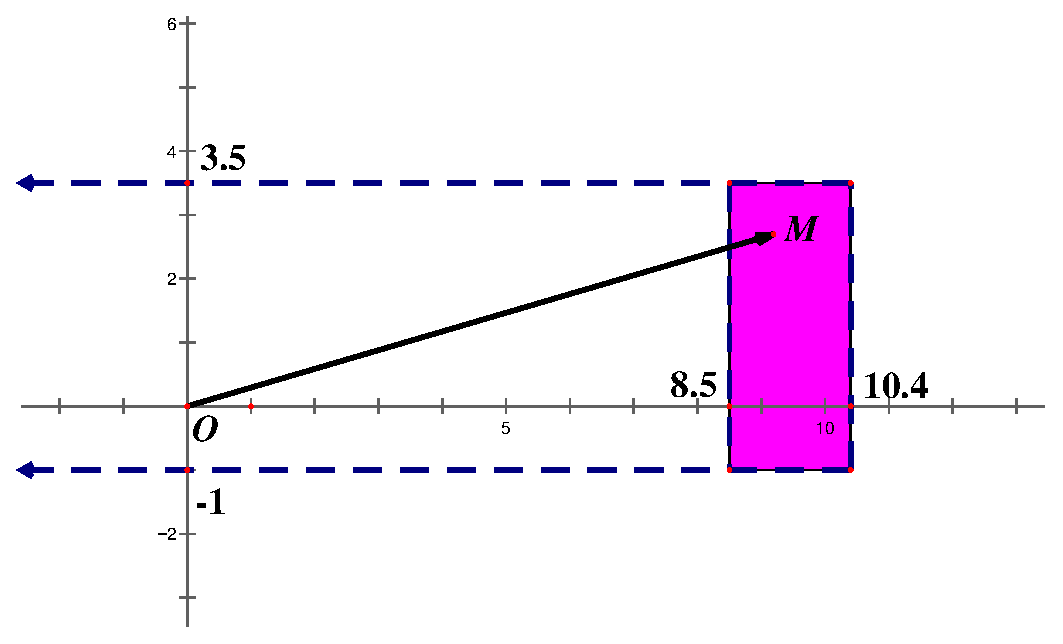
\includegraphics[width=0.9\textwidth]{images/1.eps}
\caption{雪球发射器的发射方向。O为发射点,在如图所示矩形内随机取一点M,则OM为发射方向。}\label{e1}
\end{figure}

\subsubsection{烟花火箭}
烟花神教主角。关于烟花火箭的信息请参考wiki和\url{https://www.bilibili.com/video/av5050255}。

\subsubsection{传送机}\label{chuansongji}
一个传送机分为三个图格。传送机为前景物块,可以敲成半砖。传送机的工作机制中,三个图格分别有自己的传送区域(\autoref{i216})。

\begin{figure}[!h]
\centering

\includegraphics{images/216.png}
\caption{三个图格的传送区域。如果图格被敲成下半砖,则传送区域下移半格,其他半砖形态传送区域不变。}
\label{i216}
\end{figure}

当一根电线激活时,记录下该电线下第一个结算的传送机图格与最后一个结算的传送机图格\footnote{同一根电线上的结算顺序请参阅\autoref{jiesuanshunxu}},然后将两个图格传送区域内的可传送目标互换,互换后它们的速度不变,位置相对于传送区域不变。当两个图格的传送区域有重合并且第一个图格不低于最后一个图格时无法传送\footnote{这解释了为什么传送机不会自身传送。};当两个图格的传送区域有重合并且第一个图格低于最后一个图格时可以传送,此时两传送区域重叠部分属于第一个图格的传送区域(\autoref{i217:218})。

\begin{figure}[!h]
\begin{center}
\subfloat{
\label{i217}
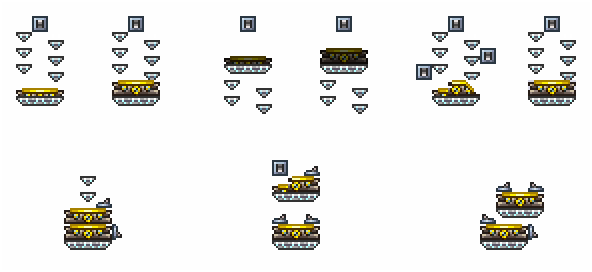
\includegraphics[width=0.9\textwidth]{images/217.png}
}
\qquad
\subfloat{
\label{i218}
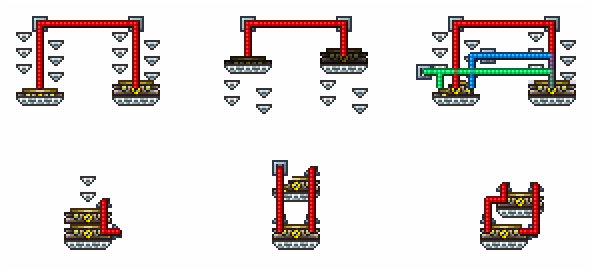
\includegraphics[width=0.9\textwidth]{images/218.png}
}
\end{center}
\caption{左上装置:右边传送机比左边传送机传送区域高半格,因此玩家从左边传送到右边会高半格。中上装置:只要碰撞箱与传送区域有一点重叠,就可以传送。右上装置:传送机的三个图格各自有传送区域,从左边传送到右边,激活绿线会高半格,而激活蓝线红线不会。下方三个装置:激活上面开关不会传送,激活下面开关会传送;传送时只要玩家在下方传送机的传送区域内,就会被从下传到上;传送时只有玩家在上方传送机的传送区域内并且不在下方传送机的传送区域内,才会被从上传到下。}
\label{i217:218}
\end{figure}

\subsubsection{像素盒}
像素盒可随意摆放,无需支撑块或背景墙。像素盒有十字状态的分线盒的分线效果。当一个电源激活时,该电源上的所有电线激活,此时如果像素盒上有横向电线激活且无纵向电线激活,那么像素盒熄灭;如果像素盒上既有横向电线激活又有纵向电线激活,那么像素盒点亮;如果无横向电线激活,那么像素盒不响应。

需要注意的是,像素盒的响应是对电源敏感的,即分别结算每个电源发出的信号,这与传送机对电线敏感不同。同时,与一般的光源在亮灭之间切换不同,像素盒响应总是调整到对应状态。

\subsubsection{矿车轨道交叉点}
交叉点上必须有两个方向的平滑轨道,那么这两个平滑轨道必定是一个覆盖另一个,此时激活交叉点会使两个平滑轨道的覆盖关系改变。需要注意的是激活交叉点可以产生的变化数量远远小于使用锤子可以产生的变化数量。

\subsubsection{其他用电器}
剩余的用电器在wiki之外的信息相当少,因此不专门介绍。它们是:雕像、烟花喷泉、烟花盒、泡泡机、呆萌气球机、派对中心、喷泉、八音盒、烟囱、天塔柱、广播盒、制动器、传送带、彩线灯泡、增速轨道。